\chapter{Analysis of the ported \textsc{BaseX} Android version}
\label{cha:analysis}
The present chapter outlines how the migrated \textsc{BaseX} Android database has been analyzed.
The focus at this part concentrates on the evaluation and the performance of the library and its ability to be a possible database for mobile devices.
First the specifications of the test devices are described and an estimation is made to show how the performance of the various devices differ.
Therefore different benchmarks have been executed to approximate the distinctive hardware properties and their execution times.
In the next chapter it is shown that the migrated database works without errors and failures on the Android mobile platform using a real device, while benchmarking the \textsc{BaseX} Android library.
These benchmarks have also been used to identify the performance of the \textsc{BaseX} Android library. 
Therefore an XML benchmark set, which is especially designed to test the performance of XQuery executions, has been used.
In aspects of performance, \textsc{BaseX} has been compared to the default Android database SQLite3 and a predication, which database system should be preferred for a specified use case, has been made.
At the end of this chapter the constraints, in terms of maximal database sizes, of the Android version of \textsc{BaseX} used in the Android operating system has been inquired.

\section{Evaluation of the test devices}
\label{sec:evaluation-of-the-test-devices}
For the measurement of the performance and the evaluation two different devices have been used.
First, for benchmarking and evaluating the \textsc{BaseX} mobile version an Android Tablet PC Samsung Galaxy Tab 2 10.1 has been utilized.
Second, for benchmarking the normal \textsc{BaseX} desktop version a Lenovo Thinkpad laptop has been used.
Both not only vary in their operating system, they also have very different hardware specifications.
Their important technical specifications can be seen in Table~\ref{tab:test-dev-specs}.
\begin {table}[htpb] 
  \centering
\begin {tabular} {|r|r|r|r|r|r|}
  	\hline
	Device&CPU&RAM&filesystem&operating system\\
	\hline
	Laptop&Intel Core2 Duo CPU L7100&2 Gb&ext4&Arch Linux\\
	&1.2 GHz&&&(3.12.0)\\
	\hline
	Tablet&Dual-core Cortex-A9&1 Gb&ext4&Android\\
	&1 GHz&&&(4.0.3)\\
	\hline
\end {tabular}
\caption {The technical specifications of the two devices, that were used for benchmark testing.}
\label {tab:test-dev-specs}
\end {table}
\newpage
Looking at this table it can be seen that the only similarity of both systems is that they are using the same filesystem, which is ext4, which is short for \textit{fourth extended filesystem}.
The RAM of the laptop is the double amount of the tablet devices available RAM and both devices have a dual core CPU with around 1 GHz.
Even if the specifications are not differ that much on the first look, their performance varies in some factors.
Therefore a measurement of the input/output (I/O) and CPU speed of both devices has been made in Section~\ref{sec:evaluation-of-the-test-devices} to get a clearer look how the devices differ.


%\section{Evaluating the working \textsc{BaseX} Android port}
%\label{sec:evaluating-the-working-basex-android-port}
%\textbf{TODO}\\
%In this section will be shown that the created \textsc{BaseX} Android port works and fit all requirements.
%For this purpose the given JUnit tests were been migrated to Android too.
%This shows that all functions work like they work on the standard Java version.
The two devices which have been used to benchmark \textsc{BaseX} are totally different and not just in the fact that one is a laptop and the other a tablet PC.
They differ in many hardware aspects, but there are two additional factors, that are interesting to identify a systems speed and are used for the given purpose.
These are the CPU speed and the input/output (I/O) speed, where I/O speed is a headline for different operations.
Broadly speaking it can be said that the I/O speed can be divided into read and write operations.\\
To measure these values the benchmark tool Bonnie++\footnote{\url{http://www.coker.com.au/Bonnie++/}} is used.
This tool executes different operations and measures how many of these operations can be executed in one second.
It tests sequential output, sequential input, random seeks, sequential create and random create.\\
The sequential output represents the write speed of the system and Bonnie++ uses three different methods to measure this value.
First it writes one character after another by using the \textsf{putc()} systemcall. 
After this operation it writes whole blocks with the size of 8192 bytes by using the \textsf{write()} systemcall and than calling the \textsf{close()} systemcall.
The last test in this category is the rewrite test and differs from the write test in the fact, that the file is not closed after writing.
Therefore one block write comply with 8192 \textsf{putc} calls and is way more effective and faster than writing single characters.
As a next test the random seek operations per seconds were measured, which means how often the read/write position can be changed.
It also measures the latency which represents the rotation speed of the disk, but this is obsolete because both systems using flash storage.
Therefore there is no revolution per minute to measure.\\
Bonny is implemented in the C++ programming language and is available on most Linux distributions.
But to use it on Android it is necessary to initially build it from its sources by using the, already mentioned in Chapter~\ref{sec:migration:the-android-project-structure}, Android Native Development Kit (NDK).
This provides a cross compiler which makes it possible to build C++ code for the Android platform.
For the execution of the benchmarks Bonnie++ in the version 1.96 has been used.
The results of these test executions can be seen in table~\ref{tab:bonnie-results-out}.
%\begin {table}
%\begin {tabular} {|r|r|r|r|r|r|r|r|r|r|r|r|r|}
%	\hline
%		&\multicolumn {3} {|c|} {Sequential}&\multicolumn {2} {|c|} {Sequential}&Random&\multicolumn {3} {|c|} {Sequential}&\multicolumn {3} {|c|} {Random}\\
%		&\multicolumn {3} {|c|} {Output}&\multicolumn {2} {|c|} {Input}&Seeks&\multicolumn {3} {|c|} {Create}&\multicolumn {3} {|c|} {Create}\\
%	\hline
%		&K/sec&K/sec&K/sec&K/sec&/sec&/sec&/sec&/sec&/sec&/sec&/sec&/sec\\
%	\hline
%	Laptop&201&62180&23850&907&98239&1161&17134&137752&13032&19442&170028&11774\\
%	\hline
%	Tablet&5&20828&8756&596&23768&475.6&39&361&167&42&391&238\\
%	\hline
%	\hline
%	Factors&40.20&2.99&2.72&1.52&4.13&2.44&439.33&381.58&78.04&462.90&434.85&49.47\\
%	\hline
%\end {tabular}
%\caption {Results of the Bonnie++ benchmarks.}
%\label {tab:bonnie-results}
%\end {table}


\begin {table}[htpb] 
  \centering
\begin {tabular} {|r|r|r|r|r|r|r|}
	\hline
		&\multicolumn {3} {|c|} {Sequential}&\multicolumn {2} {|c|} {Sequential}&\multicolumn {1} {|c|}{Random}\\
		&\multicolumn {3} {|c|} {Output}&\multicolumn {2} {|c|} {Input}&\multicolumn {1} {|c|}{Seeks}\\
	\hline
		&Char&Block&Rewrite&Char&Block&\\
	\hline
	Laptop&201K&62180K&23850K&907K&98239K&1161\\
	\hline
	Tablet&5K&20828K&8756K&596K&23768K&475.6\\
	\hline
	\hline
	Factors&40.20&2.99&2.72&1.52&4.13&2.44\\
	\hline
\end {tabular}
\caption {Results of the Bonnie++ in- and output benchmarks.}
\label {tab:bonnie-results-out}
\end {table}


Bonnie++ also measures the sequential and random create of a file.
Therefore it creates a file, queries its status and deletes it by using the POSIX systemcalls \textsf{creat()}, \textsf{stat()} and \textsf{unlink()}.
The results of this test can be seen in Table~\ref{tab:bonnie-results-create}
\begin {table}[htpb] 
  \centering
\begin {tabular} {|r|r|r|r|r|r|r|}
	\hline
		&\multicolumn {3} {|c|} {Sequential}&\multicolumn {3} {|c|} {Random}\\
		&\multicolumn {3} {|c|} {Create}&\multicolumn {3} {|c|} {Create}\\
	\hline
		&creat()&stat()&unlink()&creat()&stat()&unlink()\\
	\hline
	Laptop&17134&137752&13032&19442&170028&11774\\
	\hline
	Tablet&39&361&167&42&391&238\\
	\hline
	\hline
	Factors&439.33&381.58&78.04&462.90&434.85&49.47\\
	\hline
\end {tabular}
\caption {Results of the Bonnie++ sequential/random create benchmarks.}
\label {tab:bonnie-results-create}
\end {table}


%\begin {table}
%\begin {tabular} {|r|r|r|r|r|r|r|}
%	\hline
%		&\multicolumn {3} {|c|} {Sequential}&\multicolumn {2} {|c|} {Sequential}&\multicolumn {1} {|c|}{Random}\\
%		&\multicolumn {3} {|c|} {Output}&\multicolumn {2} {|c|} {Input}&\multicolumn {1} {|c|}{Seeks}\\
%	\hline
%		&Char&Block&Rewrite&Char&Block&\\
%	\hline
%	Laptop (per seconds)&201K&62180K&23850K&907K&98239&1161\\
%	\hline
%	Tablet (per seconds)&5K&20828K&8756K&596&23768K&475.6\\
%	\hline
%	\hline
%	Factors&40.20&2.99&2.72&1.52&4.13&2.44\\
%	\hline
%\end {tabular}
%\caption {Results of the Bonnie++ benchmarks.}
%\label {tab:bonnie-results}
%\end {table}


By analyzing these values it can be said that the laptop is overall faster than the tablet PC.
It is well known that I/O operations are the most expensive ones for use on Android, so the achieved result is no surprise. 
But with these values it can be said that there are factors which can tell how much faster it is in specific operations.
This factors are impossible to optimize, because they are a hardware constraint and only changing the hardware can effectively improve them.
But they are still important to identify the bottlenecks of the mobile \textsc{BaseX} version.\\
Analyzing Table~\ref{tab:bonnie-results-create} and having a look at the factors shows one value which is, compared to the others, extremely high.
The sequential write per character is 40 times faster on the laptop than on the tablet PC.
Considering this, it is clear to avoid writing by character instead by block.
Writing by using the block mechanism is just three times slower than on the tablet device.
The sequential reading of a single character is at the tablet just 1.52 times slower than the at the notebook.
Though the factor of the block reading is quite higher than the character reading factor it is sure to use the block reading because it is much faster than character reading.
But by using block reading the factor needs also to be considered in the \textsc{BaseX} benchmarks later in chapter~\ref{sec:analysing-the-execution-performance}.
\\
Looking at Table~\ref{tab:bonnie-results-create} it can be seen that the sequential/random creation, reading and deleting is very slow on the Android device compared to the laptop.
Considering this it should be avoided to often create files, because this type of operation is very slow.\\
Bonnie++ gives a good overview about how fast the two system handle their I/O operations and how they differ in this type of aspect.
But there is also another factor which affects the execution speed of a program, namely the CPU speed.
It is obvious that this also differs on both test devices.
To evaluate the CPU times a Java program has been written which executes four different CPU intensive operations.
First it does the naive factorial of 5000, where naive means that it just iterates till 5000 and multiplies every step to the result.
The second test is a recursive calculation of the 100th Fibonacci number.
The third sorts an ascending ordered array of 10000 items using the bubble-sort algorithm.
This is done because this is the worst case for the bubble-sort algorithm which has a complexity of $\mathcal O(n^2)$.
The last test performs a naive test if the number 666667 is prime or not, by testing to divide the number by every possible candidate step by step till the candidate is the square root of the number.
All these tests are very intensive in their CPU usage, because they only use arithmetic operations.
The test have been implemented in the C programming language and have been compiled also using the Android NDK.
The reason for this is that there is no distortion caused by the Dalvik or Java virtual machine.
The results of these tests can be seen in Table~\ref{tab:cpu-results}.
\begin {table}[htpb] 
  \centering
\begin {tabular} {|l|r|r|r|r|}
	\hline
		&Factorial&Fibonacci&Bubble Sort&Prime Number\\
	\hline
	Laptop&&&&\\
	(avg. on 1000 runs)&98.19 ms&248.63 ms&180.53 ms&15.85 ms\\
	\hline
	Tablet&&&&\\
	(avg. on 1000 runs)&491.15 ms&2336.35 ms&1045.52 ms&76.41 ms\\
	\hline
	\hline
	Factors&5&9.4&5.8&4.8\\
	\hline
\end {tabular}
\caption {Results of the CPU benchmarks.}
\label {tab:cpu-results}
\end {table}


Except the Fibonacci test it can be said that the CPU of the laptop is about five times faster than the one of the tablet device, respectively calculates and executes instructions five times faster.
This is like the different I/O parameters a factor which could not be improved and has to be considered in the \textsc{BaseX} benchmarks as well.
In general it can be said, that every operation, which is mainly CPU intensive, is executed five times faster on the laptop than on the tablet device.
The same applies to IO operations, depending on the type of the operation the laptop is up to  4 times faster than the tablet device.
These evaluations are used for measuring the performance of the two \textsc{BaseX} versions and how to cope with the results achieved by two different platforms on two different devices.

%\newpage
\section{Analyzing the Execution Performance}
\label{sec:analysing-the-execution-performance}
To investigate the performance of the Android version of \textsc{BaseX} the benchmark suite \textit{XMark} has been used.
\textit{XMark} creates random XML files and provides a set of twenty predefined queries which can be used to measure the execution performance of an \textit{XQuery} implementation.
It offers the possibility to choose the size of the randomly created XML files, so that the test queries can be executed on different file sizes.
Therefore it is also being used to search for the maximum supported database size of an \textsc{BaseX} database on Android in Section~\ref{sec:defining-the-constraints}.
All benchmark tests have been executed using the \textsc{BaseX} Android library and not the client/server solution.
Additionally the Android benchmarks have all been executed inside the main thread of an application, which is usually not the case because all database operations should be handled inside a separate thread.
The reason for this is to avoid unpredictable interrupts which could possibly hinder the benchmark thread. 
This is not the case if all benchmarks are executed inside the main thread.


\subsection{The XMark Benchmark Suite}
\label{subsec:the-xmark-benchmark-suite}
The XMark benchmark suite is used to identify the execution speed of the \textsc{BaseX} Android version.
Therefore it offers 20 different XQuery queries which are especially designed to benchmark an XQuery implementation.
The queries are separated into different categories, where every category targets a specific aspect of query execution.
The XML files that can be generated by using XMark are all containing the same elements and every file is well-formed.
The content of the generated XML files is randomly generated by using the 17000 most frequently used words\footnote{ignoring all stop words} in the plays of Shakespeare~\cite{schmidtxmark}.
The structure of the randomly generated XML files can be seen in Figure~\ref{fig:xmark-file-structure}.
\begin{figure}[htpb]
\begin{center}
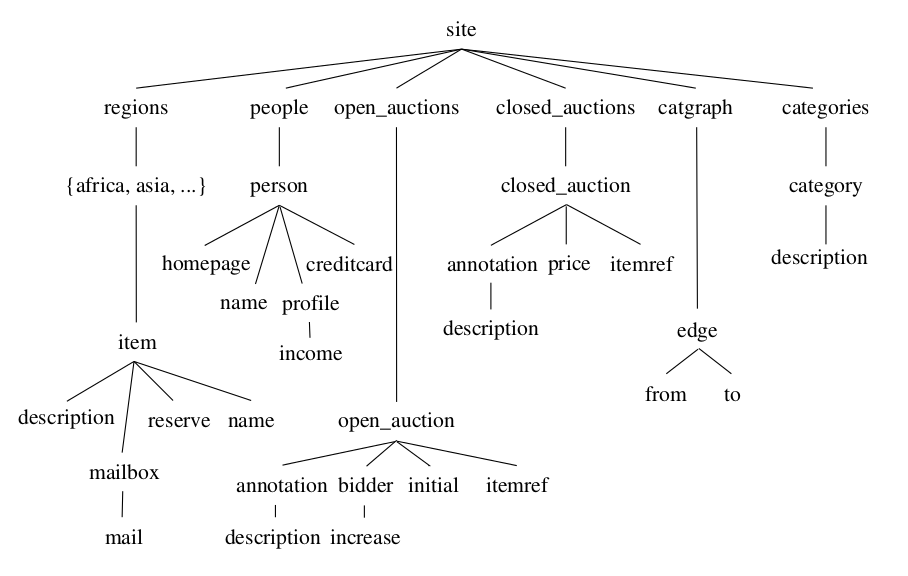
\includegraphics[scale=0.42]{images/xmark-file-elements.png} 
\caption{The structure of a generated XMark XML file. Source:\cite{schmidtxmark}}
\label{fig:xmark-file-structure}
\end{center}
\end{figure}
\newpage
The size of the XML files can be chosen during the generation process of XMark.
For testing \textsc{BaseX} 15 different files have been generated.
The smallest with a size of 100 Kb, followed by files with a size increasing by 100 KB steps.
Hence, the biggest generated file has a size of 1.4 MB.\\
The textual explanation of the different types of queries can be seen in Table~\ref{tab:xmark-queries}.
\begin {table}[htpb] 
  \centering
	\begin{tabular}{r|l}
	  \hline
	  1&Return the name of the person with ID 'person0'.\\
	  \hline
	  2&Return the initial increase of all open auctions.\\
	  \hline
	  3&Return the first and current increase of all open auctions whose current\\
	  &increase is at least twice as high as the initial increase.\\
	  \hline
	  4&List the reserves of those open auctions where a certain person issued\\
	  &a bid before another person.\\
	  \hline
	  5&How many sold items cost more than 40.\\
	  \hline
	  6&How many items are listed on all continents?\\
	  \hline
	  7&How many pieces of prose are in our database?\\
	  \hline
	  8&List the names of persons and the number of items they bought.\\
	  &(Joins person, closed\_auction)\\
	  \hline
	  9&List the names of persons and the names of items they bought in Europe.\\
	  &(Joins person\_auction, item)\\
	  \hline
	  10&List all persons according to their interest; use French markup\\
	  &in the result.\\
	  \hline
	  11&For each person, list the number of items currently on sale whose\\
	  &price does not exceed 0.02\% of the person's income.\\
	  \hline
	  12&For each richer-than-average person, list the number of items currently\\
	  &on sale whose price does not exceed 0.02\% of the person's income.\\
	  \hline
	  13&List the names of items registered in Australia along with\\
	  &their description.\\
	  \hline
	  14&Return the names of all items whose description contains the word 'gold'.\\
	  \hline
	  15&Print the keywords in emphasis in annotations of closed auctions.\\
	  \hline
	  16&Return the IDs of those auctions that have one or more keywords\\
	  &in emphasis.\\
	  \hline
	  17&Which persons don't have a homepage?\\
	  \hline
	  18&Convert the currency of the reserve of all open auctions to\\
	  &another currency.\\
	  \hline
	  19&Give an alphabetically ordered list of all items along with their location.\\
	  \hline
	  20&Group customers by their income and output the cardinality of each\\
	  &group.\\
	  \hline
	\end{tabular}
	\caption {The XMark queries. Source:\cite{schmidtxmark}}
\label {tab:xmark-queries}
\end {table}


The queries are divided into various categories, which are aiming to benchmark several functionalities and concepts of XML.
Category one includes just Query 1 and tests the performance of an exact match.
The second category analyzes the behavior of the database by querying it with order constraints.
This category contains the queries 2, 3 and 4.
Casting is the purpose of the third category, which only includes Query 5.
The next category contains the queries 6 and 7, and tests the regular path expressions.
Chasing references is the topic of the fifth category that contains Query 8 and 9.
Constructing new elements and querying them is the purpose of the next category that includes only Query 10.
Benchmarking the execution of queries with a large result set by using joins is the goal of the seventh category, which involves Query 11 and 12.
Query 13 is the only query in the next category, which aims to test the performance of reconstruction of a document.
Search a full text by using a key word is the purpose of category 9 that just includes Query 14.
The next category tests the performance of deep path traversals without wildcards, this includes the Queries 15 and 16.
Category 11 includes Query 17 and investigates the performance of the database by querying missing elements.
User defined functions are the content of the next category which only contains Query 18.
To investigate the performance of the database executing a query that sorts the result is the purpose of category 13 which is achieved by Query 19.
The last category is used to test the speed of an execution of a simple aggregation by using the last query~\cite{schmidtxmark}.

\subsection{The Results of the Benchmark Execution}
\label{sec:the-results-of-the-benchmark-execution}
To execute the XMark queries two applications have been developed, one for testing the \textsc{BaseX} desktop version and one for the Android version.
These two programs are pretty much the same except for the target platform and the used \textsc{BaseX} version.
Both feature the same functionalities while they operate equally.
At the first step the programs create 15 databases and add the 15 XML files, that were mentioned in the section before, to these databases.
After this operations the application opens one database after another and executes every XMark query on it.
Every query is executed a hundred times and the average time consumption is being calculated and stored into a specific file.
The result of the execution of the application using the laptop can be seen in Figure~\ref{fig:xmark-laptop} and the result of the execution using the tablet is shown in Figure~\ref{fig:xmark-tablet}.

\begin{figure}[!ht]
  \begin{center}
  \begin{gnuplot}[terminal=pdf, terminaloptions=color, scale=1.1]
          set title 'Laptop Steps'
	  set datafile separator ','
	  set xlabel 'Query'
	  set ylabel 'Average time in ms (100 executions)'
	  set xrange [0:21]
	  set xtics 1,1,20
	  set logscale y
	  set grid ytics lt 0 lw 1 lc rgb '#bbbbbb'
	  set grid xtics lt 0 lw 1 lc rgb '#bbbbbb'
	  set key samplen 2 spacing .5 font ',8'
	  show grid
	  set style fill solid 0.8 border -1
	  set boxwidth 0.5 relative
	  plot for [i=1:14] 'benchmarks/basex-steps-laptop-transposed.csv' u ($0+1):i title ''.i.'00kb' with linespoints
	\end{gnuplot}              
	\caption{The results of the XMark benchmark queries executed on the laptop device.}
	\label{fig:xmark-laptop}
	\end{center}
\end{figure}
\newpage
\begin{figure}[!ht]
  \begin{center}
  \begin{gnuplot}[terminal=pdf, terminaloptions=color, scale=1.1]
          set title 'Tablet Steps'
	  set datafile separator ','
	  set xlabel 'Query'
	  set ylabel 'Average time in ms (100 executions)'
	  set xrange [0:21]
	  set xtics 1,1,20
	  set logscale y
	  set grid ytics lt 0 lw 1 lc rgb '#bbbbbb'
	  set grid xtics lt 0 lw 1 lc rgb '#bbbbbb'
	  set key samplen 2 spacing .5 font ',8'
	  show grid
	  set style fill solid 0.8 border -1
	  set boxwidth 0.5 relative
	  plot for [i=1:14] 'benchmarks/xmark-tablet-steps-transposed.csv' u ($0+1):i title ''.i.'00kb' with linespoints
	\end{gnuplot}              
	\caption{The results of the XMark benchmark queries executed on the tablet device.}
	\label{fig:xmark-tablet}
	\end{center}
\end{figure}

Looking at both images it can be seen that with an increasing size of an addressed database also the execution time of the performed test queries increases.
This behaves as expected, because all queries have a complexity of at least $\mathcal O(n)$ and with an increase of the file size the amount of elements are also increasing.
It is also shown that the curves of both images are similar to each other, which is a sign for the fact that no unpredictable circumstances have occurred.
A query which is very fast on one device and the slowest on the other or vice versa would be an example for this.\\
Although the two graphics are looking very much alike they differ in one important aspect, the fact that the execution time is up to seventy times higher using the tablet PC instead of the laptop device.
Even if this factor is just the highest one, the queries which are executed using the tablet are around thirty times slower, on average, than the ones executed on the laptop.\footnote{The complete results of all executed XMark benchmark tests of the laptop and the tablet device are shown in Appendix~\ref{app:the-xmark-results}. A specific table is also given which includes the factors that show how the various execution times differ from each other.}
This results are giving a first overview of the performance of \textsc{BaseX} running on the Android platform.
The perception that \textsc{BaseX} is faster executed on the Laptop was anticipated, by just considering the lack of hardware resources at the Tablet shown in Section~\ref{sec:evaluation-of-the-test-devices}.
Remembering the fact that, for example, the CPU speed is about five times faster on the laptop than on the tablet PC it still needs some investigation on how such factors, like the seventy times higher execution time, are being achieved.
Another interesting insight is the fact that the execution time is sometimes faster using a bigger database than a small one.
This only affects the benchmarks made using the tablet device.
In general it cannot be said how the circumstances mentioned above actually occur.
Hence, more research needs to be done with the Android version of \textsc{BaseX}, which is shown in the next section.

\subsection{Identifying the Bottlenecks}
\label{sec:identifying-the-bottlenecks}
With the Android SDK various development tools are provided.
On of them is Traceview, which offers the possibility to record a specific part as source code of an execution of an application.
Traceview provides a graphical view to analyze this records or the possibility to transform them into HTML code.
The content of such records implies every method call and its execution time, as well as the occupation of the CPU in percent and the amount of calls.
The execution times are given in microseconds, which are not representing the real world time, the value represents absolute CPU occupation time.
This fact makes the recorded trace-views very valuable, because no interrupts are tampering the results.\\
All twenty XMark queries have been recorded using Traceview by executing them with a database that features the size of one mega byte in total.
Most records contain a very long list of method calls, even if they only record a small part of the code.
Therefore only the top five time consuming methods for every query have been investigated.
Summing up those methods it can be said that there is an amount of twenty methods which apply to the group of the top five time consuming methods that have been recorded using Traceview.
Traceview also records the amount of calls that every method experienced.
With this additional information it is possible to calculate the average time spend inside one method.
Table~\ref{tab:tob-five-cycle-call} shows the five methods which feature the highest values as a result of this calculation.
\begin{table}[htpb]
	\centering
	\begin{tabular}{|c|c|}
		\hline
		${cycle \over calls}$&Name\\[0.9ex]
		\hline
		32592&dalvik/system/VMDebug.startGC\\
		\hline
		1121&util/Compress.unpack\\
		\hline
		277&value/node/DBNode.uri\\
		\hline
		175&query/path/IterStep\$1.next\\
		\hline
		105&util/Token.norm\\
		\hline
	\end{tabular}
	\caption{The five methods with the highest${cycle \over calls}$ value.}
	\label{tab:tob-five-cycle-call}
\end{table}

The most time consuming method is, as shown in Table~\ref{tab:tob-five-cycle-call}, \textsf{VMDebug.startGC}.
This function is called only once and executes a long time in average.
According to~\cite{vmdebug-startgc} this method is a fake method. 
It is implemented to display the execution of the garbage collector of the Dalvik virtual machine on the Traceview records.
Unlike most implementations of the Java virtual machine, it is not possible for the Dalvik VM to change the garbage collector strategy.
It is possible to increase the size of the process's own heap, which indirectly affects the garbage collection, by slowing it down with a bigger heap size.
The available heap is hereby device dependent and increasing the size can cause crashes of the application, with out of memory exceptions.
More about the specific heap size of an application, executed on the Tablet, is described in Section~\ref{sec:analyzing-the-hardware-usage}.
Since Android version 2.3, which is the minimum version for the use with \textsc{BaseX} Android library, the garbage collector is implemented in a concurrent way and does not influence the executing thread~\cite{dubroy2011memory}.
This is also the reason why it is executed only once and its execution takes so long.
The GC thread is started for one time and collects all unreferenced objects till the process is finished.
Therefore this method is being ignored, because increasing the heap size is not an option and the garbage collector is not executed within the thread which benchmarks the \textsc{BaseX} code.

%\subsection*{Analyzing the \textsf{Compress.unpack} method}
%\label{sec:analyzing-the-compress.unpack-method}
Looking at those methods, the \textsf{DBNode.uri} method is the only one of those, which provides a possible way to be optimized.
This is done by modifying the corresponding Java source code.
Unfortunately, this method is not the top time consuming method.
\textsf{Compress.unpack} is the slowest executed method, that was recorded using Traceview.
It consumes an average of 1121 cycles per call, which is very slow compared to the other methods.
The purpose of this method, inside \textsc{BaseX}, is to decompress the given byte array.
During its execution it iterates over the given byte array and decompresses all characters.
\\
The \textsf{IterStep\$1.next} method is part of an iterator and each time iterates to the next node.
Depending on the amount of nodes, the time spend in this method and the corresponding calls to it can in- or decrease.
This results in the conclusion that this method could also not be optimized for the Android operating system.
\\
\textsf{Token.norm} is used to normalize all whitespaces in the byte array which is passed using the parameter of this method.
By normalizing it is meant to search for horizontal tabs, line feeds, carriage returns and spaces inside the byte array and then replaces them by an empty character.
This is done in a normal for-loop and could also not be improved by changing it.
The only method, that has the potential to be optimized by modifying the corresponding Java source code is the \textsf{DBnode.uri} method, which is shown in the following section.


\subsection*{Analyzing the \textsf{DBNode.uri} Method}
\label{sec:analyzing-the-dbnode.uri-method}
The third most time consuming method is the \textsf{DBNode.uri} method with an average of 277 cycles per call.
Listing~\ref{lis:uri-code} shows the corresponding source code for the \textsf{NSGlobal.uri} method.
\lstset{language=Java,
   basicstyle=\footnotesize,
   keywordstyle=\color{blue!80!black!100},
   identifierstyle=,
   commentstyle=\color{green!50!black!100},
   stringstyle=\ttfamily,
   breaklines=true,
   numbers=left,
   tabsize=2,
   numberstyle=\footnotesize,
   frame=single,
   backgroundcolor=\color{blue!3},
}
\begin{lstlisting} [captionpos=b, caption={The code for the uri method in the NSGlobal class.}, label=lis:uri-code] 
public byte[] uri(final byte[] pref) {
    if(stack != null) {
      for(int s = stack.size() - 1; s >= 0; s--) {
        if(eq(stack.name(s), pref)) return stack.value(s);
      }
    }
    final byte[] uri = staticURI(pref);
    return uri == null ? NSGlobal.uri(pref) : uri.length == 0 ? null : uri;
}
\end{lstlisting}
		
%An answer to this question could be that the amount of the iterations of the for loop is the highest value it can be, because nothing more happens in the loop and its complexity is $\mathcal O(n)$.
Looking at the source code for the \textsf{uri} method shows that it only executes a for-loop and checks if the parameter \textsf{pref} is equal to the \textsf{NS.name} byte and if this is the case the value is returned.
The method has a complexity of $\mathcal O(n)$ which results in the assumption that the for-loop is always executed in the worst case.
This would mean that every time the method is called the loop is fully iterated from the maximum size of the \textsf{NS} object till zero.
Considering the, in Section~\ref{sec:migration:comparison-of-the-two-virtual-machines} mentioned, Just In Time compiler from the Dalvik VM this part of code should be optimized by it.
Even if this part of the \textsc{BaseX} Android source code is compiled into native machine code it is still very slow, compared to the other expensive methods.
Besides the for-loop there are the \textsf{eq} and \textsf{NS.name} methods, which also could produce the long execution time of this function.
The \textsf{eq} method compares the two committed byte arrays for equality, implemented by using a for-loop which iterates over the arrays and compares their bytes.
This for-loop is executed very often and there are no other method calls inside of it, so it is very obvious that this loop is compiled into machine code by the JIT optimization routine.\\
The investigation of the \textsf{NS.name} method shows that this function is a just simple getter method which returns the name from the index of the parameter.\\
At this place the differences between the two platforms are playing an important part, because it is a best practice to use getter and setter for the normal Java environment, but it is expensive for the Android platform~\cite{toninievlautatingandroid}.
Even if the JIT compiler inlines the getter/setter calls it can be up to 30\% faster if a direct field access is used instead of the getter/setter methods~\cite{toninianalysis}.\\
In Section~\ref{sec:improving} the getter of the \textit{NSGlobal.uri} method has been replaced by direct field accesses and it is shown that it improves the execution time of Query 2 for the \textsc{BaseX} Android library.
This has also been applied for the \textsc{BaseX} desktop version and investigated if there is also an improvement of the execution speed.

\newpage
\subsection{Analyzing the Hardware Usage}
\label{sec:analyzing-the-hardware-usage}
In Section~\ref{sec:evaluation-of-the-test-devices} it has been shown, that the laptop computes five times faster, in average, as the tablet PC.
Additionally to this the write operation on the file system is up to three times slower on the tablet compared to the laptop and the read operation is about four times faster while performed on the Laptop.
Thinking about those factors could lead to the solution that most of the longer execution times on the tablet device are achieved by the given hardware constraints.
The created Traceviews also show a often use of the \textsf{TableDiskAccess} class.
This class offers methods to store the data on the disk or to read it, therefore it uses block-wise operations.
The measured values of Section~\ref{sec:analyzing-the-hardware-usage} for the I/O operations on the test devices, illustrates that writing is three times faster on the laptop than on the tablet PC.
And reading is even more than four times faster compared to the Tablet device, by using block wise operations.
For the XMark benchmark test a write operation has not been significantly executed, because the benchmarks only query the data and does not create new one which is stored permanently in the database.
Therefore no Traceview shows the usage of the \textsf{writeBlock} method for example, the analyzing of the write performance of the \textsc{BaseX} Android library is shown later in this section.\\
In contrast to the write operation, the read operation is used very often.
Even if it is not part of the most time consuming methods in the Traceviews it is still the factor of four which always needs to be considered, when it is being executed.\\
To measure the performance of the write operation an Android application has been created which creates databases and fills them with different data.
The provided data has been created using the given XMark tool to create random XML files.
Therefore files with a size of 1, 5 and 10 MB have been generated.
As well as testing the Android version of \textsc{BaseX}, in its write ability, the desktop version has also been tested with the same set of data.
The results can be seen in Table~\ref{tab:average-times-create-db}.
\begin{table}[htpb]
	\centering
	\begin{tabular}{|c|c|c||c|}
		\hline
		File size&Laptop&Tablet&Factor\\
		\hline
		1 Mb&168.54 ms&3389.55 ms&20.11\\
		\hline
		5 Mb&737.88 ms&17418.61 ms&23.60\\
		\hline
		10 Mb&1543.37 ms&36246.68 ms&23.48\\
		\hline
	\end{tabular}
	\caption{The average times of the create database operation, for 50 runs.}
	\label{tab:average-times-create-db}
\end{table}

The results of the measured write operations illustrate that the laptop in average is about twenty times faster in writing operations than the tablet device.
To narrow it down, why this big factor occurs while creating a database on the tablet PC, the Traceviews for the create database operation have also been recorded.
The Traceviews have been recorded using all three file sizes, but they all have the same ordering of top time consuming methods and they differ only in their execution times and calls.
Therefore the 1 Mb example has been used for analyzing the recorded Traceview.\\
Looking at the top five most time consuming methods inside the Traceview of the create operations shows that all of them are read and not write operations.
The reason for this is that \textsc{BaseX} spends the most of the time inside a create process to parse a given XML file, due to flat table representation~\cite{grun2010storing}.

\begin{table}[htpb]
	\centering
	\begin{tabular}{|c|c|}
		\hline
		${cycle \over calls}$&Name\\[0.9ex]
		\hline
		5.69&XMLInput.read\\
		\hline
		5.46&XMLScanner.consume\\
		\hline
		5.70&TextInput.read\\
		\hline
		5.67&NewlineInput.read\\
		\hline
		5.50&TextDecoder\$UTF8.read\\
		\hline
	\end{tabular}
	\caption{The five methods with their ${cycle \over calls}$ value for the create operation.}
	\label{tab:top-five-cycle-call-write}
\end{table}

Analyzing the top time consuming methods, gives an average ${cycle \over calls}$ of a factor of around five, which is nearly the same for every method, as shown in Table~\ref{tab:top-five-cycle-call-write}.
This also applies for the Traceviews of the create operation of the 5 and 10 MB file size databases, where their number of cycles increase as well as their amount of calls.
Also analyzing the code of those methods does not provide any possibility to effectively improve their performance.\\
\\
The Android operating system has a process management which is optimized for mobile devices with low resources.
Android provides two different types of available RAM. 
First the private one, which is only available for the application itself, and secondly the shared RAM which is split between the running applications.
The process management suspends processes which are not being executed to the background and if there is a lack of available RAM it starts to kill those processes and free their memory till enough RAM is available again.
This can not be affected by the application itself.
Therefore it cannot be measured how much RAM is in use by the actual executed application and which is occupied by other processes that operate in the background.
The same applies to the available CPU usage, depending on the decisions of the operating system the application receives CPU time or not.
These constraints are also playing a role in classifying the performance of the \textsc{BaseX} Android library, because those are factors which cannot be influenced directly.\\
The Android Development Kit provides its application developer a tool that offers the possibility to view log messages during the execution of an application.
This tool is called Logcat and can be used in combination with the Android Debug Bridge.
The used garbage collector inside the Dalvik virtual machine always prints a message to the Logcat when it starts to free memory.
This information can be used to receive an overview on how often the garbage collector is triggered and how much memory it frees.
The information displayed are the reason for the garbage collection, the freed amount of memory, the heap stats and the time needed for the garbage collection by itself.\\
Depending on the available heap size of the process this output varies for every execution, due to the memory management mechanism of Android.
However, the Logcat output of the garbage collector for Query 5 and Query 11 has been recorded.
Query 5 is the query with the least amount of time consumption and Query 11 is in contrast to this the most time consuming query.
This fact is also reflected in the corresponding output of the Logcat information.
Namely the garbage collector is called only one time by the execution of Query 5 on a 1 Mb database and freed an amount of 540 KB in total, pausing the execution for 6ms.
In contrast to this minimal usage of the GC the messages shown by the Logcat during the execution of Query 11 are showing an amount of 25 of GC usage.
The values summed up can be seen in Table~\ref{tab:gc-stats}.

\begin{table}[htpb]
	\centering
	\begin{tabular}{|c|c|c|c|}
		\hline
		Query&GC executions&Freed memory&Time used\\
		\hline
		5&1&540 kb&6 ms\\
		\hline
		11&25&15173 kb&226 ms\\
		\hline
	\end{tabular}
	\caption{Garbage collection statistics during the execution of Query 5 and 11.}
	\label{tab:gc-stats}
\end{table}

This illustrates that the garbage collector of the DVM also slows down the execution of \textsc{BaseX} on the Android platform.
The last column of the table displays hereby the real time which the application is paused due to garbage collection.
The garbage collector is executed within its own thread which is scheduled by the Android operating system and needs an average time consumption of 40 ms for every execution.\\
Usually the available RAM for every process is between 16 and 128 MB.
At the used tablet device an executed application receives 48 MB of RAM for its execution, which compared to typical desktop systems is very low.
However, there is a way to increase this size manually for applications which are needing a bigger RAM size.
This can be done in the Android Manifest file by adding \textit{android:largeHeap="true"} and resulting in a total of 256 Mb RAM available for the \textsc{BaseX} application on the Tablet test device.
The increase to a maximum of 256 MB of available heap size does not mean that the application has this amount as default available.
Actually it means that the application can request more heap if it is running low on it and the operating system will grant it until the maximum capacity of 256 MB is reached.
Additionally this option is only used for testing purpose, because it is just available for Android versions higher or equal than API level 11 and therefore cannot be written from within the Manifest file of the \textsc{BaseX} Android library.\\
The result of the test is that the artificial increasing of the heap size has not effected the garbage collection of \textsc{BaseX} Android library, because only small objects are being allocated actually.
The purpose of the option to increase the heap size is to load large objects into the heap, which under normal circumstances would run out of memory, for example with the use of large bitmaps.
Although \textsc{BaseX} allocates a lot of memory, but it does not keep it, the garbage collector frees it due to the fact that the allocated objects are not be used any more.
This also is a reason for the frequent occurrence of the garbage collector while executing Query 11 from the XMark benchmark suite.
And this is another factor which slows down the \textsc{BaseX} Android version because of the restrictions given by the operating system and the virtual machine, which cannot be avoided.



%This is the same factor achieved by the evaluation of the test devices in Section~\ref{sec:evaluation-of-the-test-devices} by using block writing operations.
%This realization leads to the consumption that this value is a hardware constraint and can not be optimized by changing the source code or any other software aspect.
\newpage
\section{Differences of the Mobile and Desktop Version of \textsc{BaseX}}
\label{sec:differences-of-the-two-basex-versions}
Despite the listed differences in Sections~\ref{sec:migration:creating-a-basex-android-library} and \ref{sec:migration:problems-during-the-migration} there are more distinctions between both versions.
The Java Development Kit (JDK) offers a tool which is called Hprof.
This is similar to the Traceview tool provided by the Android SDK and offers the possibility to record the execution of a specific class or method.
The Android tool Traceview is actually an extension of Hprof that expands Hprof with some functionalities.
Unfortunately some of those functionalities have been used to identify the most time consuming methods at the \textsc{BaseX} Android version and therefore those are missing at Hprof.
This missing functionalities and the fact that Hprof is not accurate makes it not as valuable as Traceview~\cite{mytkowicz2010evaluating}.
However, Hprof provides the ability to be used to identify methods which are being executed the most.
It does not provide the CPU occupation time in cycles, like Traceview, but it displays it in overall percent and it also offers a list of the heap allocations made by the recorded program~\cite{liang1999comprehensive}.
This information can be used to identify the top time consuming methods, which can then be compared with the most top time consuming methods of the \textsc{BaseX} Android version.
The time spend in those methods and the amount of calls to those methods are not displayed, but it can be said that those methods are being compiled into native machine code by the HotSpot Just In Time compiler of the Java Virtual Machine.
As explained in Section~\ref{sec:migration:comparison-of-the-two-virtual-machines}, the JVM uses a method based JIT, that compiles the so called hot spot methods, which are the ones displayed by Hprof. 


%The differences can also be seen by identifying the traceviews of the \textsc{BaseX} desktop version.
Analyzing all Hprof dumps illustrates the additional differences between the two \textsc{BaseX} versions.
None of the top five time consuming methods of the recorded Traceviews from Section~\ref{sec:identifying-the-bottlenecks} are actually represented inside the Hprof records.
Remembering the fact that the \textsf{VMDebug.startGC} method is part of the Dalvik virtual machine, which is responsible that it is not represented in any record of the Hprof runs.
The second most time consuming method of the benchmarks of the Android version of \textsc{BaseX} is the \textsf{Compress.unpack} method, as already shown in Section~\ref{sec:identifying-the-bottlenecks}.
This method is also represented as one of the top time consumers inside the Hprof records for the desktop version.
The \textsf{DBNode.uri} method was the third most time consuming method in the Android version before its improvement.
At the desktop version of \textsc{BaseX} it is also listed in the recorded Hprof executions, but it is not one of the slowest methods.
This also underlines the differences between the mobile and the desktop version, because at the not improved Android version this method marks one of the existing bottlenecks.
As mentioned in Section~\ref{sec:analyzing-the-dbnode.uri-method} the Just In Time compiler of the Dalvik virtual machine could be a reason for such a behavior.
In contrast to this the JIT of the Java virtual machine seems to translate the getter calls to native machine code, which can be an explanation why the \textsf{DBNode.uri} method is not in the top time consuming methods of the Hprof records.
Except for this difference no other significant differences in the Traceviews of the \textsc{BaseX} Android and the desktop version have been extinguished.
Additionally to this there is a small distinction between the two platforms, which is not listed in the most time consuming method.
There are several input/output methods in the Traceviews of the Android version which are not listed that high inside the Hprof records.
A possible explanation for this is the faster I/O operation speed of the hardware of the laptop device compared to the hardware of the tablet PC, as shown in Section~\ref{sec:evaluation-of-the-test-devices}.\\
The analysis and comparison of the Hprof records and the Android Traceviews are underlining the assumption that most of the bad execution performance achieved by the \textsc{BaseX} Android version is caused by the lack of hardware resources on the given mobile device.




%Nevertheless, the second most time consuming method in the Android version of the benchmark tests, the \textsf{Compress.unpack} method, is also not represented in one of the Hprof records.
%In fact no method of the class \textsf{Compress} is represented in the Hprof records for all XMark queries.

%Compared to the desktop version this class often provides methods which are represented in the most time consuming methods in the Android version.\\
%The \textsf{DBNode.uri} method was the third most time consuming method in the Android version before the improvement.
%In the desktop version of \textsc{BaseX} it is also listed in the recorded Hprof executions, but it is not one of the slow methods.
%This also illustrates the differences between the mobile and the desktop version, because at the not improved Android version this method is one of the bottlenecks.
%Looking at benchmarks of the desktop version this method is not significant slower than other methods.
%This circumstance is also a proof that the change for the improvement of the Android version has no effect on the desktop version of \textsc{BaseX} and illustrates again the difference between the two virtual machines and their JIT compilers.\\
%Looking at the table in Section~\ref{sec:identifying-the-bottlenecks} gives the \textsf{IterStep\$1.next} method as fourth time consuming method in the Android version.
%This method is also represented in the same test queries as a time consuming method.
%In this aspect the two versions are similar to each other, both have a similar amount of calls to the method.
%The times spend in this method can not be compared, because of the lack of information in the Hprof records.\\
%The last of the top five time consuming methods of the not improved Android version is the \textsf{Token.norm} method.
%This one does also not significantly occur in the Hprof records, but contrary to the \textsf{Compress.unpack} method it is listed in the records.\\
%\\




\section{Results of the Improvement}
\label{sec:improving}
%In this section is shown how the found bottlenecks can be improved and the time consumption of some functionalities are made better.
One aspect which was found as a possible improvement, by analyzing the execution times and the corresponding Traceviews from Section~\ref{sec:identifying-the-bottlenecks}, is the getter and setter part.
As mentioned in Section~\ref{sec:analyzing-the-dbnode.uri-method} the use of direct field access instead of getter/setter methods improves the execution time by 30\%.
This value is shown by Tonini\cite{toninievlautatingandroid} and is the change which has been done for the \textsc{BaseX} Android library.
The recorded Traceviews have shown that especially the \textsf{DBNode.uri} method features a high execution time caused by the getter calls inside the for-loop.
This call accesses the \textsf{nm} byte array which is one part of tuples of name and value pairs in the container class \textsf{Atts}.
All calls to the getter and setter to these tuples have been replaced by direct field accesses inside the whole \textsc{BaseX} Android library.\\
The execution of the XMark benchmark tests with this optimized version of \textsc{BaseX} on the tablet PC showed an improvement of up to 200\%, which is nearly three times faster as the normal version of \textsc{BaseX}.
Especially the time consumption for the execution of the queries 2, 10 and 17 have been improved.
An extensive use of the \textsf{DBNode.uri} method with those queries is responsible for this behavior.
The average improvement of this change is about 58.6\%.
Analyzing the Traceviews of the improved version shows, that the average execution time of the \textsf{DBNode.uri} method has been nearly cut into half and it is not even close to the list of the top time consuming methods.
The results of the whole execution can be found in Appendix~\ref{tab:xmark-tablet-optimized-appendice} and the improvements for every query in percent is illustrated inside Table~\ref{tab:improvements-percent}, which is also available in the Appendices chapter at the end of the present thesis.\\
The replacements of the getter and setter calls at the desktop version of \textsc{BaseX} have no significant changes in the time consumption of the overall execution time.
This was also tested on the laptop device, which underlines the statement that this mechanism, to speed up an application, is only working at the Android version and is the result of the used JIT from the Dalvik virtual machine.
The average improvement of 58.6\% is even higher than the 30\% mentioned before and achieved by Tonini\cite{toninievlautatingandroid}.
This shows, that the replacement of the getters/setters is a technique which need to be continued in the \textsc{BaseX} library project, as well as in every other time consuming Android application.
Responsible for the improvement on the Android platform is the, in Section~\ref{sec:migration:comparison-of-the-two-virtual-machines} and before mentioned, Just In Time compiler of the Dalvik virtual machine. 
Even if the compiler copies the getter and setter methods to the corresponding place inside the code, the JIT is not able to transform them into native code, therefore they have to be replaced with direct field accesses.
Using direct field access enables the JIT to translate those accesses into native machine code and this is responsible for the boost of time improvement.
Figure~\ref{fig:xmark-tablet-optimized} shows that the curves still have the same shape, which indicates that the changes had an impact on the whole execution of the benchmark suite.
The most time consuming queries inside the benchmark tests of the unimproved version are still the most time consuming methods in the improved version and the same applies for the fast queries.
The Queries 8, 9 and 11 are still the slowest ones, but the overall time consumption could has been lowered instead.

\begin{figure}[!ht]
  \begin{center}
	\begin{gnuplot}[terminal=pdf, terminaloptions=color, scale=1.1]
	          set title 'Tablet Steps using the Optimized Version'
		  set datafile separator ','
		  set xlabel 'Query'
		  set ylabel 'Average time in ms(100 executions)'
		  set xrange [0:21]
		  set xtics 1,1,20
		  set logscale y
		  set grid ytics lt 0 lw 1 lc rgb '#bbbbbb'
		  set grid xtics lt 0 lw 1 lc rgb '#bbbbbb'
		  set key samplen 2 spacing .5 font ',8'
		  show grid
		  set style fill solid 0.8 border -1
		  set boxwidth 0.5 relative
		  plot for [i=1:14] 'benchmarks/xmark-tablet-steps-optimized-transposed.csv' u ($0+1):i title ''.i.'00kb' with linespoints
	\end{gnuplot}              
	\caption{The results of the XMark benchmark queries executed on the Tablet, using the optimized \textsc{BaseX} version.}
	\label{fig:xmark-tablet-optimized}
  \end{center}
\end{figure}




Compared to the old execution time, the adjustment results in an enormous improvement.
However, compared to the times achieved on the laptop devices the benchmarks are still slow on the tablet device.
It is hard to tell where the most time of the execution is spend and how this affects the performance of \textsc{BaseX} on the Android operating system.
In general the Android virtual machine Dalvik is designed to be a fast VM that executes its code in less instructions than an implementation of the JVM.
The implication of this should be a faster execution of the \textsc{BaseX} code on the Dalvik VM than on the JVM.
The lesser hardware capabilities of the Tablet are playing a big role in the execution of the benchmarks, especially the available RAM for the DVM, which has been shown in the section before.
Therefore the best improvement would be more available hardware resources in order to speed up \textsc{BaseX} significantly.


\section{Comparison between \textsc{BaseX} and SQLite3}
\label{sec:comparison-between-basex-and-sqlite}
Even after an optimization of the \textsc{BaseX} Android version the execution of the XMark benchmark tests are still significantly slower than the desktop version.
It has been shown that the main part, which is responsible for this behavior, is the limited hardware resources available on mobile devices and some restrictions in use with the Dalvik virtual machine have been extinguished.
Therefore the execution times of \textsc{BaseX} are now being compared to the execution times of the SQLite3 database, which is part of Android, as already described in Section~\ref{sec:android-internals}.
SQLite3 is a relational database which uses SQL as its query language and not XQuery, which is used by \textsc{BaseX} instead.
Thus, to benchmark both database systems and compare them to each other the queries have to be very similar as well as the used data inside the databases.
The used data for the comparison of the two databases are identical and consists of a set of contacts, including the name, city, post- and email address of a person.
In the SQLite3 database all this columns are represented as string values and all have to be filled, the same applies for the database inside \textsc{BaseX}.
The structure of the respective SQLite3 table can be seen in Figure~\ref{fig:sqlite-tables-contacts}.
The corresponding XML structure used in \textsc{BaseX} in Listing~\ref{basex-xml-contacts}.

\begin{figure}[h]
\begin{center}
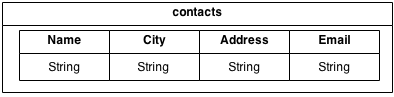
\includegraphics[scale=0.65]{images/sqlite-tables.png} 
\caption{The structure of the used table inside SQLite3.}
\label{fig:sqlite-tables-contacts}
\end{center}
\end{figure}

\lstinputlisting[captionpos=b, caption={The XML structure of the contacts database for use with \textsc{BaseX}.}, label=basex-xml-contacts, language=XML]{listings/contacts-structure.xml}


Depending on the amount of contacts eight different sizes of databases have been used for the benchmark test.
Starting from small to big the databases are containing 10, 50, 100, 500, 1000, 1500, 2500 and 5000 contacts.
There are six different statements which have been used for the benchmark purpose.
The SQL statements as well as their corresponding XQuery code can be seen in Appendix~\ref{statement1-sql}.
They are divided into  two categories; one is querying and the other is modifying the given data.
During the execution of the statements the time of their execution was measured and their exact functionality can be seen in the following list:
\newpage
\begin{enumerate}
	\item Get all contacts by their name in ascending order.
	\item Get all contacts having an email address ending with ``com''.
	\item Search for a specific name.
	\item Delete every contact having an email address ending with ``org''.
	\item Insert a new contact.
	\item Update the recent inserted contact.
\end{enumerate}
The statements listed above are not intensive statements which would be used to stress test the database, as it has been done in Section~\ref{sec:analysing-the-execution-performance} with the XMark benchmark queries.
In contrast to this the statements are easier queries which could also occur in the use case of a real application.
The benchmarks have been executed using the tablet device and the optimized \textsc{BaseX} Android library.
The consumed time of the query statements and the different databases can be seen in Table~\ref{tab:sqlite3-vs-basex-results-1}, as well as the results achieved by the modifying statements in Table~\ref{tab:sqlite3-vs-basex-results-2}.


\begin {table}[htpb] 
  \centering
\begin {tabular} {|r|r|r|r|r|r|r|}
	\hline
	&\multicolumn {2} {|c|} {Statement 1}&\multicolumn {2} {|c|} {Statement 2}&\multicolumn {2} {|c|} {Statement 3}\\
	\hline
	Contacts&SQLite3&\textsc{BaseX}&SQLite3&\textsc{BaseX}&SQLite3&\textsc{BaseX}\\
	\hline
	10&2.00&23.77&1.70&24.10&1.15&24.38\\
	50&12.14&50.81&2.44&50.57&1.38&41.74\\
	100&13.67&91.43&3.58&58.56&1.52&56.12\\
	500&28.93&149.96&9.61&100.12&2.62&276.09\\
	1000&76.41&269.65&14.92&180.38&4.05&353.94\\
	1500&79.41&401.67&25.90&308.38&5.79&435.97\\
	2500&198.57&752.74&51.66&501.06&9.73&684.26\\
	5000&419.86&1491.21&55.41&992.18&20.05&1366.02\\
	\hline
%	\hline
%	10&0.27&2.96&0.27&4.05&0.24&6.86\\
%	50&0.24&3.63&0.24&10.34&0.21&36.40\\
%	100&0.27&2.89&0.24&25.87&0.27&25.78\\
%	500&0.24&3.12&0.45&69.94&0.21&114.47\\
%	1000&0.26&3.23&0.54&182.76&0.27&316.04\\
%	1500&0.23&3.02&0.24&242.64&0.24&389.55\\
%	2500&0.30&2.83&0.57&401.33&0.30&722.68\\
%	5000&0.36&2.89&0.24&755.46&0.27&1485.41\\
%	\hline
\end {tabular}
\caption {Measured execution times for the query statements in milliseconds.}
\label {tab:sqlite3-vs-basex-results-1}
\end {table}

\begin {table}[htpb] 
  \centering
\begin {tabular} {|r|r|r|r|r|r|r|}
	\hline
	&\multicolumn {2} {|c|} {Statement 4}&\multicolumn {2} {|c|} {Statement 5}&\multicolumn {2} {|c|} {Statement 6}\\
	\hline
	Contacts&SQLite3&\textsc{BaseX}&SQLite3&\textsc{BaseX}&SQLite3&\textsc{BaseX}\\
	\hline
	10&4.39&9.67&32.65&9.85&4.18&10.16\\
	50&4.91&21.11&28.32&11.01&4.27&14.22\\
	100&28.77&22.76&32.44&9.67&4.33&32.19\\
	500&355.49&88.19&52.67&10.32&5.43&80.96\\
	1000&728.27&178.00&41.17&10.23&5.92&111.81\\
	1500&972.47&311.06&72.33&10.22&6.43&192.90\\
	2500&1357.69&570.00&152.85&10.28&7.29&253.44\\
	5000&2270.29&1016.99&364.71&15.96&10.65&594.90\\
	\hline
\end {tabular}
\caption {Measured execution times for the modify statements in milliseconds.}
\label {tab:sqlite3-vs-basex-results-2}
\end {table}

Looking at the results of the query statements in Table~\ref{tab:sqlite3-vs-basex-results-1} illustrates the speed advantage of SQLite3 compared to \textsc{BaseX}.
On both database systems the time consumption depends on the amount of used data and there is nearly a linear growth in every query on both databases.
Overall, the general result is that SQLite3 is faster in every query statement than \textsc{BaseX}.
In query 1 it is between three and four times faster, in query 2 it is around 20 times faster and executing statement 3 is around 60 times faster using SQLite3.\\
%The size of the database is not important for SQLite, while \textsc{BaseX} increases its execution time for statement 2 and 3 with the rising size of the database.
%Looking at statement 1 illustrates that both database systems have a constant execution time by just querying the whole data and ordering it.\\
In contrast to the query results the values of Table~\ref{tab:sqlite3-vs-basex-results-2} are showing that inserting and deleting of data is both faster with \textsc{BaseX} than with the use of SQLite3.
Deleting all data with an \textit{org} ending in their email is nearly twice as fast using \textsc{BaseX} instead of SQLite3.
Inserting a new contact into the database is always performed in a constant time using \textsc{BaseX}, while it increases with the size of the database using SQLite3.\\
The fast query times are one advantage of SQLite3, the reason why this is achieved is that SQLite3 is specially implemented for mobile devices.
Similar to the \textsc{BaseX} Android version, SQLite3 does not use a client/server architecture and therefore every application has its own database\cite{wei2012android}.
SQLite3 is a system library of Android, it is implemented in the C programming language and therefore needs no virtual machine for its execution, which makes it faster in the aspect of time consumption.
Another reason for the fast execution of every query is the use of a buffer cache, which is used by SQLite3 and cannot be disabled to measure the absolute performance of the database~\cite{kim2012androbench}.
Making a query in SQLite3 on an Android device also returns a cursor object pointing to the first result and not the whole result. 
To receive the whole result, as a string for example, the received cursor is used to iterate through the results.
For this comparison the same has been done with \textsc{BaseX}, an iterator object is the result of a query and not as usual a string containing the results.
This saves the time and resources which would be used to build the result as one single string.\\
\\
In the XMark benchmark tests the whole results, received by a query, have been whole strings.
This fact is also partial responsible for the achieved execution times.
As mentioned before, to get a result as a string the received cursor of a SQLite3 query has to be used to iterate over the result set.
To get an overview how \textsc{BaseX} and SQLite3 handle the queries by returning the whole result as a string this has also been measured and the results can be seen in Table~\ref{tab:sqlite3-vs-basex-results-3}.

\begin {table}[htpb] 
  \centering
\begin {tabular} {|r|r|r|r|r|r|r|}
	\hline
	&\multicolumn {2} {|c|} {Statement 1}&\multicolumn {2} {|c|} {Statement 2}&\multicolumn {2} {|c|} {Statement 3}\\
	\hline
	Contacts&SQLite3&\textsc{BaseX}&SQLite3&\textsc{BaseX}&SQLite3&\textsc{BaseX}\\
	\hline
	10&3.90&45.10&1.31&56.94&1.12&25.32\\
	50&41.44&49.22&2.13&27.40&1.37&35.49\\
	100&108.33&108.85&4.63&52.52&1.52&50.47\\
	500&1891.66&203.27&75.19&95.61&2.99&247.65\\
	1000&7996.00&272.09&383.75&219.11&4.05&306.33\\
	1500&17040.43&426.26&886.87&355.22&5.58&450.59\\
	2500&56181.91&831.93&2540.80&566.83&8.51&703.73\\
	5000&211718.96&1684.96&9407.74&1090.27&15.59&1316.77\\
	\hline

\end {tabular}
\caption {Measured execution times for the query statements returning the result as a string in milliseconds.}
\label {tab:sqlite3-vs-basex-results-3}
\end {table}

The results displayed in Table~\ref{tab:sqlite3-vs-basex-results-3} illustrate, depending on the size of the result, that \textsc{BaseX} achieves a still tolerable time with 1.6 seconds by querying 5000 datasets and receiving it as a string.
In contrast to this SQLite3 is during the execution of the same operation around 200 times slower, which is caused by the part of building the string by iterating over the returned result set.
The table also displays the correlation between the required time and the size of the string.
This applies to both SQLite3 as well as \textsc{BaseX}.
Query 1 returns all contacts, while query 3 only returns one record and therefore is faster, because of a smaller result iterator and the consequent result string.
Even if query 3 just returns one record and query 1 5000, the time consumption of both queries using \textsc{BaseX} are differing by just 300 milliseconds.
The same applies for the smaller databases, \textsc{BaseX} processes the queries in nearly the same time.
For the described use case, this constitutes an advantage of \textsc{BaseX} over SQLite3, because there is no worst or best case of the queries.
The execution time just depends on the size of the database and not, as it is in SQLite3, on the size of the received results.


Those results are illustrating that applications that consist of many queries should use SQLite3 and otherwise applications with an huge insert and delete ratio should prefer \textsc{BaseX} as their database system.
At this conclusion it need to be considered how the results of a query should be handled, if they are iterated later or if they should being displayed after receiving them from a query as a single string, for example.
For the last circumstance \textsc{BaseX} should be preferred, because querying and receiving the whole result as a string is still fast compared to SQLite3.

Looking at some results of all tables in the given section shows that there are sometimes variations in the linearity of the results.
An example for this is the insertion of a contact in the database with the size of 50 contacts using \textsc{BaseX}, as shown in Table~\ref{tab:sqlite3-vs-basex-results-2}.
There can be more than one possible clarifications for this circumstance.
One could be the execution of the garbage collector at the given moment, or another interrupt of the operating system has been executed.
The Android process management, as described in Section~\ref{sec:android-internals}, makes it impossible to avoid such interrupts and therefore those erratic fluctuations. 


Unfortunately it was not possible to compare \textsc{BaseX} with the XQuery processor MXQuery, mentioned in Section~\ref{sec:overview:related-work}, which should also be available for the Android operating system.
The reason for this is that it seems that MXQuery will not be further developed since its initial release back in 2011.
The Android version of MXQuery uses an old library of Apache Xerces\footnote{\url{http://xerces.apache.org}} as its XML parser, which is deprecated and not supported by Android any more.
Therefore it could not have been compared to the \textsc{BaseX} Android version, and makes \textsc{BaseX} the only available XML database and XQuery processor for Android, at the moment.

%An example scenario could be applications for collecting a huge amount of data, because the more data is collected the bigger the size of the database will get.
%And the constant time of inserting data into the database is hereby a big plus.
%In contrast to this, applications with a big database and a lot of searches inside this database should use SQLite3, because even the search operation is constant at this database system.
%
\newpage
\section{Defining the Constraints of the \textsc{BaseX} Android Version}
\label{sec:defining-the-constraints}
On mobile devices there are not as many hardware resources available as on desktop computers.
Therefore in this section the constraints have been searched, which are representing the maximal boundaries for using the \textsc{BaseX} database in a mobile environment.\\
However, the great variety of Android devices makes it nearly impossible to make a general statement about the constraints of \textsc{BaseX}, because of their different hardware capabilities.
Thus, the tablet device has also been used to estimate the constraints of \textsc{BaseX}, which results in the fact that found restrictions are not applying for other devices.\\
To find the first constraint, which is the maximum size of a \textsc{BaseX} database, different XML files have been created using the XMark tool, explained in Section~\ref{subsec:the-xmark-benchmark-suite}.
Their sizes start by 50 MB and also increases by 50 MB steps.
Every step a new database is created and the specific file is added to the database.
If the previous step was successful the first five queries of the XMark benchmark suite will be executed on this specific database.
The reason for using the first five queries is that those are not so intensive and complex, but they still represent a good example how it could be found in a real application.
The selected results can be seen in Table~\ref{tab:basex-constraints}.

\begin {table}[htpb] 
  \centering
\begin {tabular} {|r|r|r|r|r|r|r|}
	\hline
	Size&Create&Query 1&Query 2&Query 3&Query 4&Query 5\\
	\hline
	50 MB&222.7&1.1&3.3&4.4&4.2&1.3\\
%	60 MB&278.2&1.0&2.3&5.0&5.0&1.6\\
%	70 MB&327.2&1.1&3.1&6.0&5.9&1.9\\
%	80 MB&391.7&1.7&3.4&6.7&6.7&2.3\\
%	90 MB&407.8&1.4&3.7&7.7&7.6&2.6\\
       100 MB&484.5&1.6&3.7&8.3&8.2&2.6\\
%       110 MB&501.4&3.0&4.2&9.1&8.8&2.8\\
%       120 MB&564.5&1.8&6.0&9.7&9.5&2.9\\
%       130 MB&599.6&2.2&5.1&11.8&11.8&3.8\\
%       140 MB&636.8&2.7&6.0&12.7&12.8&3.8\\%836.8
       150 MB&669.0&2.7&6.0&13.4&13.7&4.2\\
%       160 MB&778.7&3.5&6.3&13.4&13.2&4.3\\
%       170 MB&842.8&3.4&6.6&14.8&15.5&5.0\\
%       180 MB&878.1&4.5&7.7&14.3&14.9&4.7\\
%       190 MB&884.4&4.6&7.5&15.7&15.4&5.0\\
       200 MB&984.0&5.4&10.5&17.9&18.1&5.9\\
       250 MB&1169.5&5.2&9.7&20.3&20.5&6.7\\
       500 MB&2447.5&8.5&19.1&45.3&41.2&13.3\\
       \hline
      % ..\\
       \hline
       2 GB& 8712.8&37.9&81.2&219.5&167.3&22.8\\
	\hline
\end {tabular}
\caption {Measured execution times, in seconds, while creating large databases and subsequently querying them.}
\label {tab:basex-constraints}
\end {table}
The displayed results of Table~\ref{tab:basex-constraints} illustrate that creating a large database is combined with a create time effort. 
Looking at the required times to create each database, shows a linearity which increases about 200 seconds with 50 MB is shown.
The query times are illustrating that \textsc{BaseX} is not a choice for applications with many queries combined with a large database in mobile environments, at the moment.
However, the results are still proving that it is possible to use \textsc{BaseX} to handle a large database, for mobile devices, in the Android environment.
The largest file size, which has been used to find the maximal size of a database, was 2 GB.
\textsc{BaseX} needed more than 2.5 hours to create and around 40 seconds to execute Query 1 on the 2 GB database on the Tablet.
This is a very long time, but thinking about the dimensions of this file illustrates how this times have been achieved.
The 2 GB XML file contains more than 35 million elements, which is not common for the use with mobile devices.
% and would usually be stored on an external server and can therefore be used with the client version of \textsc{BaseX}, created in Section~\ref{sec:migration:providing-a-server-client-solution}.
Compared to this amount of elements, the used XML contacts files in Section~\ref{sec:comparison-between-basex-and-sqlite} with 20.000 elements\footnote{5000 contact nodes each with 4 elements} has a file size of around 1 MB.
Even if there will be no application, in the near future, which uses this amount of data to store with the \textsc{BaseX} Android version it has been shown that it is theoretically possible.
In addition to this, it has to be said that the device needs enough free space to create the database in its internal storage indeed.\\
Additionally to the supported maximum storage size it is not possible to find a minimal CPU and RAM size, because of the huge variety of available Android devices.
It can be assumed that if a device has enough hardware resources to run the Android operating system, it also provides enough resources to use the \textsc{BaseX} Android library.\\
In general it can be said if a device has enough hardware resources it is also possible to use the \textsc{BaseX} Android version with large databases, but it would violate the principles of mobile devices.
To avoid this disruption, it is common sense to handle databases with such an amount of data on an external server.
Those data could then be accessed and modified with the client version of \textsc{BaseX}, created in Section~\ref{sec:migration:providing-a-server-client-solution}.


%The circumstance that the used 2 GB XML file has more than 35 million elements and \textsc{BaseX} is still able to create and query a database of this size is responsible for the definition of 2 GB as a maximal supported files size.
%The only aspect is the amount of time spend to create and query those big databases, but it is still possible.


